\chapter{Werkzeuge für effiziente Code-Entwicklung}
In diesem Kapitel werden die verwendeten "Werkzeuge" näher erläutert, die bei der Code-Entwicklung unterstützt haben. Dabei wird auch auf Aspekte der Vorlesungsreihe Effizient programmieren \cite{Kessler.Sommersemester2017} eingegangen.

\section{Entwicklungsumgebung und Versionsmanagement}
Wie in \cite{Kessler.Sommersemester2017} beschrieben können Entwicklungsumgebungen bei der Entwicklung und Implementierung von Programmen unterstützen. Aufgrund des Windows-Betriebssystems ist die Entscheidung auf  Microsoft Visual Studio 2017 gefallen. Für die Reproduzierbarkeit wurde ein Repository bei GitHub angelegt. Da es sich bei dieser Arbeit nicht um ein Gruppenprojekt handelt, wurde lediglich ein Trunk angelegt. Es wurde stets darauf geachtet, dass die Version nur comitted und gepushed wurde, wenn das Programm lauffähig war und zuvor getestet wurde \cite{Kessler.Sommersemester2017}.  
\section{Code Dokumentation}

\section{Verwendung von Open Source Bibliotheken}
\label{sec:OSBib}
Nach  \cite{Kessler.Wintersemester201718}  ist es nicht immer notwendig bei gewissen Funktionalitäten immer bei Null zu beginnen, sondern auf bereits bestehendes Aufzubauen.
Da in dieser Arbeit die Simulation im Vordergrund steht und nicht die Implementierung von grundlegenden Funktionen, wurden neben den C++ Standardbibliotheken ebenfalls Open Source Bibliotheken eingebunden. Aufgrund dessen, dass besagte Simulation auf dem Matlab Programm nach \cite{Olucak.15.02.2017} beruht, ist die Lineare Algebra unverzichtbar. Zudem wurden Daten häufig in komprimierten .mat-Files gespeichert.\newpage Es liegt also nahe diese grundlegenden Funktionen mithilfe von bereits vorhanden Bibliotheken nach Möglichkeit abzudecken.
\\Die in diesem Projekt verwendeten Open Source Bibliotheken werden in Tabelle \ref{tab:openSource} kurz beschrieben.
\begin{table}[h]
	\centering	\begin{tabular}{l p{10cm}}
		\textbf{Name der Bibliothek} & \textbf{Kurzbeschreibung}\\
		Eigen &  C++ Template Bibliothek für lineare Algebra \cite{TuxFamily.2018}\\\\
		matio & C/C++ Bibliothek, die Funktionen bereitstellt, um Daten aus und in .mat-Files zu lesen/schreiben
	\end{tabular}
	\caption{Übersicht über verwendete Open Source Bibliotheken}
	\label{tab:openSource}
\end{table}\\
Wie aus \ref{tab:openSource} ersichtlich handelt es sich bei der Eigen-Bibliothek um Templates. Nachdem Eigen in das Programm eingebunden wird, kann sofort auf die Funktionen zugegriffen werden. Zum Einlesen der .mat-Files wurden aufbauend auf den  Funktionen aus der matio-Bibliothek selber eine Klasse implementiert, die diese Funktionalität bereitstellt. Um matio zu verwenden werden sei darauf verwiesen, dass zusätzlich noch die Bibliotheken HDF5 und zlib benötigt werden. 



\chapter{Simulations-Framework}
\label{ch:Simulations-Framework}
Im Nachfolgenden Kapitel soll die Grundidee des Simulations-Frameworks erläutert werden. Zum Einen soll ein modularer Aufbau umgesetzt werden, sodass im späteren Verlauf die Module nach dem Baukastenprinzip zu einer Gesamtsimulation zusammengesetzt werden. Zum Anderen soll der Nutzer in der Lage sein, in den Modulen verschiedene Methoden zu nutzen, ohne dabei den Code zu verändern.
\section{Aufbau der Module}
\label{sec:AufbauModule}
Jedes Modul beschreibt eine spezifische Domäne des Flugzeuges und  besitzt mehrere Klassen, die im Nachfolgenden allgemein erläutert werden. Eine Klasse ist für die Auswahl und den Aufruf der gewünschten Modelle zuständig und besitzt den gleichen Namen wie das Modul (Modulklasse). Sie wird im späteren Verlauf in der Simulation aufgerufen und dient sozusagen als Schnittstelle zu den anderen Modulen. Um nun eine gewünschte Methoden aufrufen zu können, ohne dabei den Code zu verändern, wird auf das Prinzip der Vererbung  zurückgegriffen.  Die Kind-Klassen können von der Elternklasse oder von einem Kind abgeleitet werden. Der allgemeine Aufbau eines Moduls wird in Abbildung \ref{fig:UML_Modul} dargestellt.
 \begin{figure}[h]
 	 \centering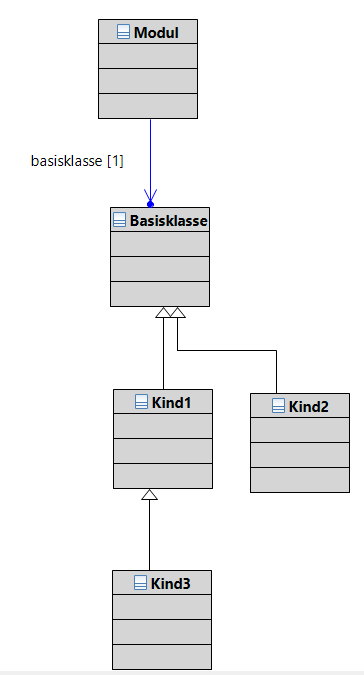
\includegraphics[width=0.23\linewidth]{UML_Modul.PNG}
 	 \caption{Allgemeiner Aufbau eins Moduls }
 	 \label{fig:UML_Modul}
 \end{figure} \newpage
Zusätzlich besitzen alle Klassen neben Konstruktor und Destruktor auch Standard-Methoden, die in Tabelle \ref{tab:Standardmethoden} beschrieben werden.\\
\begin{table}[h]
	\centering	\begin{tabular}{l p{10cm}}
		\textbf{Standard-Methode} & \textbf{Bedeutung}\\
		init(...) & Die für die jeweilige Domäne benötigten Parameter werden aus den Input-Files eingelesen und Variablen initialisiert.\\\\
		update(...) & Methode in der die eigentliche Berechnung/Simulation der spezifischen Domäne für jeden Zeitschritt durchgeführt wird
	\end{tabular}
	\caption{Standard-Methoden der Simulation}
	\label{tab:Standardmethoden}
\end{table}\\
Die Standard-Methoden sollen einen einheitlichen Funktionsaufruf gewährleisten. Neben besagten Standard-Methoden können die Klassen auch noch zusätzliche Methoden besitzen, worauf später noch näher eingegangen wird. \\
Im Speziellen wird hier Polymorphie mithilfe von virtuellen Funktionen genutzt. Dazu werden die Standard-Methoden der Basisklasse als virtuelle Funktionen deklariert, was exemplarisch im Listing \ref{list:Basisklasse} zu sehen ist.

\begin{lstlisting}[label = {list:Basisklasse}, caption = Aufbau des Header-Files der Basisklasse,captionpos=b]
...
	virtual initBasisklasse();

	virtual updateBasisklasse();
...
\end{lstlisting}
Aus diese Grund lässt sich die Basisklasse auch als polymorphe Klasse bezeichnen \cite{Wolf.2014}. \\
Um nun zu gewährleisten, dass das gewünschte Modell des Moduls ausgewählt wird, wird ein ein Basisklassenzeiger verwendet. Der Zeiger kann auf jedes Objekt adressiert werden, dass von ihm abgeleitet wurde. Die eigentliche Initialisierung findet in der Modulklasse statt. Dazu wird neben den Standard-Methoden noch die Methode \textbf{SelectModuleType} implementiert, wobei \textbf{Module} für das jeweilige Modul steht. \newpage
\begin{lstlisting}[label = {list:ModulAuswahl}, caption = Basisklassenzeiger im Modul.cpp File ,captionpos=b]
void Modulklasse::SelectModuleType(int Type)

switch(Type){
	case 1:
		BasePtr= new Kindklasse1;
		break;
	
	case 2: 
		BasePtr = new Kindklasse2;
		break;
}

\end{lstlisting}
Durch das Schlüsselwort \textbf{virtual} in der Basisklasse wird der Compiler veranlasst, zum entsprechenden Objekt die dazugehörige Methode aufzurufen, wenn das Objekt über den Zeiger auf die Basisklasse angesprochen wird. \\
Im nächsten Schritt können nun in der Modulklasse die Standard-Methoden der Basisklasse aufgerufen werden, wie im Lisiting \ref{list:ModulAufruf} dargestellt.
\begin{lstlisting}[label = {list:ModulAufruf}, caption = Aufruf der Standard-Methoden  im Modul.cpp File ,captionpos=b]
void Modulklasse::initModulklasse()
{
	BasePtr->initBasisklasse();
}

void Modulklasse::updateModulklasse()
{
	BasePtr->updateBasisklasse();
}
\end{lstlisting}

Somit können die Methoden der Kind-Klassen, wo die Modelle implementiert wurden, aufgerufen werden, in dem die Standard-Methoden der Modulklasse aufgerufen werden. Der Nutzer muss lediglich den spezifische Modell-Parameter im Input-File ändern, um ein anderes Model auszuwählen.
\newpage
\section{Aufbau und Ablauf der Ausbaustufen}
\label{sec:Ausbaustufen}
Durch die Beschreibung der Flugzeugdomänen mithilfe der Module, ist man nun in der Lage die eigentliche Simulation im Baukastenprinzip aufzubauen.\\ In Tabelle \ref{tab:Modulbeschreibungen} werden alle Module, die für die Ausbaustufen der Simulation benötigt werden, kurz umschrieben. Dabei wird lediglich die Allgemeine Funktion des jeweiligen Moduls beleuchtet, anstatt deren Implementierung, um einen Überblick zu erhalten. \\
\begin{table}[h]
	\centering	\begin{tabular}{l p{9cm}}
		\textbf{Modulname} & \textbf{Kurzbeschreibung}\\\\
		Actuator	& Simuliert die Rudermaschinen des Flugzeuges\\\\
		Aerodynamic & Die aerodynamischen Kräfte und Momente des Flugzeuges werden berechnet\\\\
		Airframe & Enthält die Bewegungsgleichungen des Flugzeuges\\\\
		Atmosphere & Hier ist die Standard-Atmosphäre hinterlegt.\\\\
		Autopilot & Hier ist die Flugregelung implementiert\\\\
		Engine & Die Triebwerke werden simuliert\\\\
		Guidance & Stellt die Lenkung zur Verfügung\\\\
		IMU & Simuliert die Inertialsensoren\\\\
		Navigation & Hier findet die Berechung der Navigationslösung für das GNC statt.
	\end{tabular}
	\caption{Module der generischen Flugzeug-Simulation}
	\label{tab:Modulbeschreibungen}
\end{table}\\
An dieser Stelle sei angemerkt, dass es noch weitere Module gibt, die allerdings vielmehr eine sekundäre Rolle für die eigentliche Simulation einnehmen. Auf besagte Module wird im späteren Verlauf dieser Arbeit noch eingegangen. Zudem sei noch erwähnt, dass nur Domänen implementiert wurden, die für eine nichtlineare flugmechanische Simulation benötigt werden. \\
Wie bereits in \ref{sec:ausgangslage} beschrieben, werden verschiedene Ausbaustufen der Simulation benötigt. Unter Ausbaustufe ist hierbei die Anzahl an Freiheitsgraden und Detaillierungsgrad gemeint. Die Ausbaustufen werden im Modul \textbf{Trajectory} implementiert. Der Aufbau und der Aufruf erfolgt wie in Abschnitt \ref{sec:AufbauModule} beschrieben. Je nach Ausbaustufe werden innerhalb des Trajektorien-Moduls die in Tabelle \ref{tab:Modulbeschreibungen}  beschriebenen Module über ihre Modulklasse aufgerufen.
Insgesamt sind drei Ausbaustufen vorgesehen, die im Folgenden erläutert werden.\newpage
Die niedrigste Ausbaustufe ist eine Simulation mit 3 Freiheitsgraden. Es werden nur die translatorischen Bewegungsgleichungen berücksichtigt. Die Aufruf-Reihenfolge wird in Abbildung \ref{fig:3Dof} aufgezeigt.
\begin{figure}[h]
	\centering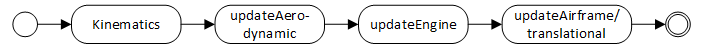
\includegraphics[width=0.8\linewidth]{3Dof.PNG}
	\label{fig:3Dof}
	\caption{Aktivitätsdiagramm der Trajektorie mit 3 Freiheitsgraden}
\end{figure}\\
Eine solche Ausbaustufe könnte beispielsweise schon sehr früh genutzt werden, wenn zum Beispiel noch keine Trägheitsmomente bekannt sind. \\
Die nächst höhere Ausbaustufe besitzt 6 Freiheitsgrade. Sie ist eine Kindklasse der zuvor beschriebenen Ausbaustufe. Der Ablauf ist in \ref{fig:6Dof} zu sehen. 
\begin{figure}[h]
	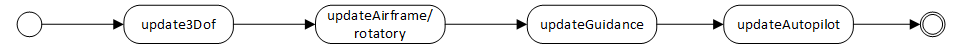
\includegraphics[width=1.0\linewidth]{6Dof.PNG}
	\label{fig:6Dof}
	\caption{Aktivitätsdiagramm der Trajektorie mit 6 Freiheitsgraden}
\end{figure}\\
Die Kindklasse wird um die rotatorischen Bewegungsgleichungen ergänzt. Außerdem erhält sie ein Flugführungssystem, das sich aus einer Lenkung und einem Flugzustandsregler zusammensetzt. In den beiden bisherigen Ausbaustufen wird das Systemverhalten als ideal angesehen. Das bedeutet, dass weder Messfehlern durch Sensorik oder Verzögerung durch Aktuatorik berücksichtigt werden. Eine solche Ausbaustufe könnte beispielsweise genutzt werden, um die Flugregelung auf dem nichtlinearen Modell zu testen und zu beurteilen. \\
Unabhängig von der Güte der physikalischen und mathematischen Modelle ist es dennoch wichtig, ab einem gewissen Grad des Entwicklungsprozesses Fehlermodelle für Subsysteme zu berücksichtigen. Somit wird eine weiter Ausbausstufe benötigt. Diese ist in Abbildung \ref{fig:realSys} zu sehen.
\begin{figure}[h]
	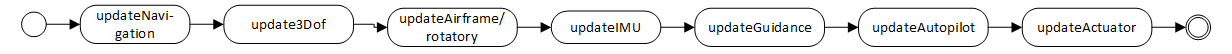
\includegraphics[width=1.0\linewidth]{realSystem.PNG}
	\label{fig:realSys}
	\caption{Aktivitätsdiagramm der Trajektorie mit 6 Freiheitsgraden unter Berücksichtigung von Fehlermodellen}
\end{figure}\\
Die höchste Ausbaustufe erbt von der zweiten Ausbaustufe. Anstatt der idealen Integration der Kinematik wird ein Naviagations-Modul verwendet. Dort wird im Regelfall eine Navigationslösung erzeugt, in dem die Sensormessungen genutzt werden um durch einen Kalman-Filter Position und Lage zu schätzen. Zudem wird die Messung durch Inertialsensoren berücksichtigt. Verzögerungen, die beispielsweise durch die Rudermaschinen verursacht werden, können im Akutator-Modul modelliert werden.

\section{Gesamtsimulation}
Die zuvor beschriebenen Ausbaustufen können genutzt werden, um die Flugbahn eines Flugzeuges zu simulieren. Somit ist es naheliegend das Gesamtflugzeug in einem eigenen Modul zu beschreiben, dem \textbf{Aircraft}-Modul.\\
Neben dem Trajektorien-Modul wird dort ebenfalls die Atmosphäre initialisiert. Der Ablauf des Gesamtflugzeuges wird in Abbildung \ref{fig:Aircraft} aufgezeigt, wobei angemerkt sei, dass sämtliche Objekte bereits initialisiert wurden.
\begin{figure}[h]
	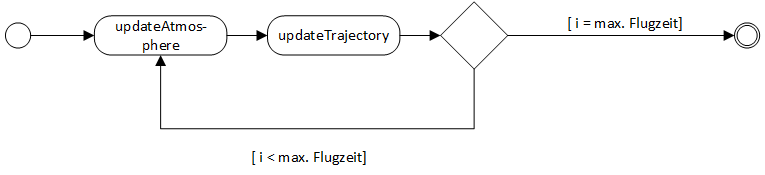
\includegraphics[width=1.0\linewidth]{Aircraft.PNG}
	\label{fig:Aircraft}
	\caption{Aktivitätsdiagramm der Gesamtflugzeug-Simulation}
\end{figure}\\
